 %% 
%% Copyright 2007-2019 Elsevier Ltd
%% 
%% This file is part of the 'Elsarticle Bundle'.
%% ---------------------------------------------
%% 
%% It may be distributed under the conditions of the LaTeX Project Public
%% License, either version 1.2 of this license or (at your option) any
%% later version.  The latest version of this license is in
%%    http://www.latex-project.org/lppl.txt
%% and version 1.2 or later is part of all distributions of LaTeX
%% version 1999/12/01 or later.
%% 
%% The list of all files belonging to the 'Elsarticle Bundle' is
%% given in the file `manifest.txt'.
%% 

%% Template article for Elsevier's document class `elsarticle'
%% with numbered style bibliographic references
%% SP 2008/03/01
%%
%% 
%%
%% $Id: elsarticle-template-num.tex 168 2019-02-25 07:15:41Z apu.v $
%%
%%
\documentclass[preprint,12pt]{elsarticle}

%\usepackage{biblatex}
\usepackage{amsmath}
\usepackage{hyperref}
\usepackage{xargs}
\usepackage[colorinlistoftodos,prependcaption,textsize=tiny]{todonotes}

%\usepackage{float,rotating,subfigure}
\newcommandx{\commentPaul}[2][1=]{\todo[linecolor=red,backgroundcolor=red!25,bordercolor=red,#1]{#2}}
%% Use the option review to obtain double line spacing
%% \documentclass[authoryear,preprint,review,12pt]{elsarticle}

%% Use the options 1p,twocolumn; 3p; 3p,twocolumn; 5p; or 5p,twocolumn
%% for a journal layout:
%% \documentclass[final,1p,times]{elsarticle}
%% \documentclass[final,1p,times,twocolumn]{elsarticle}
%% \documentclass[final,3p,times]{elsarticle}
%% \documentclass[final,3p,times,twocolumn]{elsarticle}
%% \documentclass[final,5p,times]{elsarticle}
%% \documentclass[final,5p,times,twocolumn]{elsarticle}

%% For including figures, graphicx.sty has been loaded in
%% elsarticle.cls. If you prefer to use the old commands
%% please give \usepackage{epsfig}

%% The amssymb package provides various useful mathematical symbols
\usepackage{amssymb}
\usepackage{here}
\graphicspath{{../}{../Figures/}}

\newcommand{\blue}[1]{{\leavevmode\color{blue}{#1}}} %for displaying red texts 
%% The amsthm package provides extended theorem environments
%% \usepackage{amsthm}

%% The lineno packages adds line numbers. Start line numbering with
%% \begin{linenumbers}, end it with \end{linenumbers}. Or switch it on
%% for the whole article with \linenumbers.
%% \usepackage{lineno}

\usepackage{gensymb}
\usepackage{amsmath}

\graphicspath{{../}{../Figures/}}

\journal{Solar Energy}

\setlength{\marginparwidth}{2cm}
\begin{document}

%\begin{frontmatter}


\title{Annual Antireflection Solar Module Enhancements for Fixed Modules}
%\title{Antireflection Solar Module Enhancement}



\author{Sooraj P. Sharma_1}

\address{\textsuperscript{1}University of Pittsburgh, Department of Mechanical and Materials Science, Pittsburgh, PA 15261, USA}

\author{Paul W. Leu_{1,2,3,*}}
\address{\textsuperscript{1}University of Pittsburgh, Department of Industrial Engineering, Pittsburgh, PA 15261, USA}
\address{\textsuperscript{2}University of Pittsburgh, Department of Mechanical Engineering and Materials Science, Pittsburgh, PA 15261, USA}
\address{\textsuperscript{3}University of Pittsburgh, Department of Chemical Engineering, Pittsburgh, PA 15261, USA}
\address{\textsuperscript{*}Corresponding Author: pleu@pitt.edu}


\begin{abstract}




\end{abstract}


%%
%%\begin{highlights}
%%\item Simple, clear-sky, insolation model with provided code.
%%\end{highlights}
%\begin{keyword} Antireflection, Optimization, Simulation
%\end{keyword}
%\end{frontmatter} 

%% \linenumbers

%% main text
\section{Introduction}

New antireflection coatings offer advantages of both broadband antireflection and wide angle antireflection.  
Recently, we utilized Bayesian learning optimization with finite difference time domain simulations to determine the optimized antireflection properties of single layer thin film, nanowire arrays, and nanocone arrays, which are shown in Fig.~\ref{fig:Structures} \cite{Haghanifar:20}. 
Sub-wavelength nanostructures have been of interest for their broadband and broad angle antireflection properties
\cite{Han:19,Haghanifar:20nov}.
Our simulations demonstrated that nanowire arrays and single layer thin films have comparable antireflection performance.  
The best nanowire array has an effective index of refraction similar to that of an optimized thin film with 
an index of refraction that is the geometric mean of the glass and air.  
In contrast, the nanocone arrays demonstrate superior antireflection performance where they are able to 
grade the index of refraction between the air and the glass.  
Nanocone arrays are able to achieve solar integrated normal reflection of 0.15\% and 
solar integrated 65 \degree incidence of 1.25\%.  Such structures could be created in glass via maskless reactive ion etching methods 
\cite{Haghanifar:19,Haghanifar:17} or other patterning methods \cite{Infante:13}.

Both broadband and broad angle antireflection may have benefits for solar modules, which are typically fixed installations as opposed to tracking 
due to the economic costs associated with tracking \cite{Bolinger:20}.  Fixed installations are often installed at non-ideal orientations and tilts as, for
example, the existing orientation and slope of a roof may be used. In addition, diffuse radiation
from the sky and ground reflected radiation also result in light hitting the solar module across a variety of non-normal incidence angles.
It is not clear what power generation enhancements can be expected due to these antireflection structures under different fixed and tracking configurations.  
%under different fixed and tracking
%configurations

Fig.~\ref{fig:Structures} 
shows the optimized structures previously determined from Bayesian optimization
\cite{Haghanifar:20}.
%insert figure 1 here
The single layer thin film consists of a single dielectric 
with an an index of refraction of the geometric mean of glass and air or $n_1 = 1.21$ and thickness  $t = 120$ nm. 
% Normal reflection of 0.51
% reflection at 65 degrees of 5.05 
The nanowire array has a pitch $a = 390$ nm, a diameter of $d = 290$ nm, and a height of $h = 150$ nm.
%of 390 and 290 nm, respectively.  
%diameter of  
%.  
% normal reflection of .4745
% reflection at 65 degrees of 5.77
The nanocone has a pitch $a = 400$ nm, 
bottom diameter $d_{bot} = 400$ nm, top diameter $d_{top} = 90$ nm, and height $h = 640$ nm.
% normal reflection of 0.16
% reflection at 65 degrees of 1.25
\begin{figure}[H]
\vspace{-10pt}
 \centering
 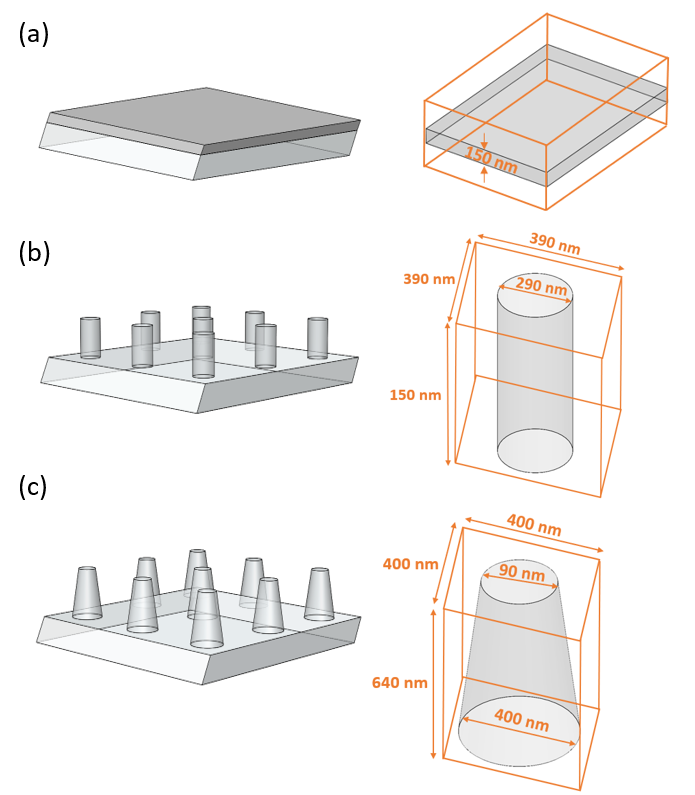
\includegraphics[width=10.5cm]{Schematic}
\caption{Structures and dimensions of the (a) thin film, (b) nanowire, and (c) nanocone simulated in this study.}
 \label{fig:Structures}
 \commentPaul[inline]{Use true dimensions in schematic}
  \commentPaul[inline]{Maybe different color than orange.}
 \end{figure}

The full reflection spectra of these these three structures were simulated by the finite difference time domain method (FDTD).  
The broadband fixed angle source technique is used to simulate the periodic structures with a broadband plane wave source illuminated at an angle
\cite{Liang:14}.
%Broadband Fixed Angle Source Technique 
The reflection spectra of various antireflection structures is shown in 
Fig.~\ref{fig:ARspectra}.
%The three optimized structures were simulated using the finite difference time domain method.  
The reflection is shown as a function of wavelength along the radius and incidence angle $\theta$ in the circumferential direction.  The reflection is shown for (a)(i) bare glass, (ii) thin film, (iii) nanowire array, and (iv) nanocone array.  
The reflection spectra shown is averaged for both TE and TM polarized light and averaged over the incident azimuth angles $\gamma_i$.
The integrated reflection as a function of incidence angle $\theta$ is shown in 
Fig.~\ref{fig:ARspectra}(b).  
The reflection spectra is integrated over the AM1.5D solar spectrum \cite{AM1p5}
for wavelengths from 280 to 1200 nm.  
The bare glass has a solar integrated reflection of 3.73\% at normal incidence
compared to 0.80, 0.64, and 0.19\% for the thin film, nanowire array, and nanocone array, respectively.  
The thin film and nanowire array have very similar antireflection performance over all the incidence angles, 
while the nanocone array also has the best antireflection properties across all incidence angles. 
At 60$\degree$ incidence angle, the solar integrated reflection is 
17.77, 4.11, 4.14, and 0.64\%, for the bare glass, thin film, nanowire array, and nanocone array, respectively.  


%\commentPaul{Maybe this should be 1.5D}

%The reflection spectra is integrated over the AM1.5G solar spectrum \cite{AM1p5}
%for wavelengths from 280 to 1200 nm.  
%\commentPaul{Maybe this should be 1.5D}


\begin{figure}[H]
\vspace{-10pt}
 \centering
 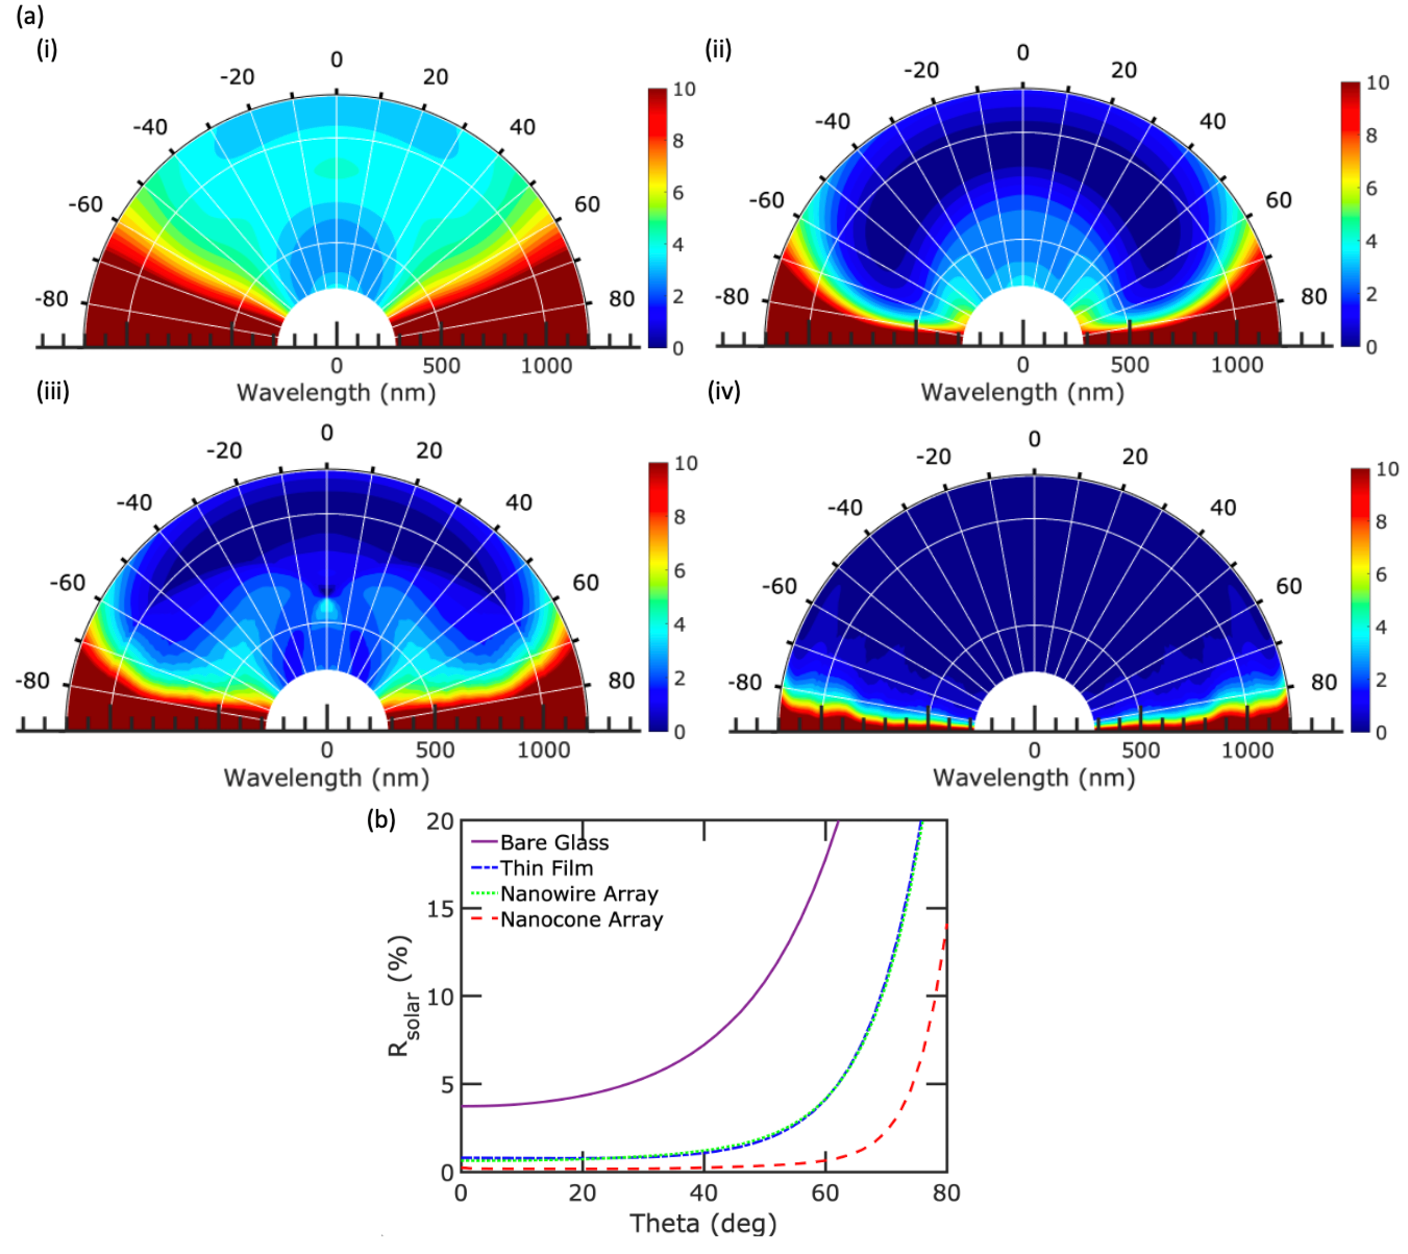
\includegraphics[width=13.5cm]{Reflection}
\caption{Reflection spectra of different structures.  (a) Reflection spectra as a function of incidence angle $\theta$ for (i) bare glass, (ii) thin film, (iii) nanowire array, and (iv) nanocone array.  
(b) Integrated solar reflection as a function of incidence angle.}
 \label{fig:ARspectra}
 \end{figure}


%\commentPaul{Please create schematic of the different structures.  You can just modify the schematic we used before but give the exact dimensions.}



% The total solar module photon flux consists of both the direct beam and the diffuse components, 
% \begin{equation}
% \Phi_{Tm} = \Phi_{bn} \cos \theta + \frac{1 + \cos \beta}{2} \Phi_{d}   
% \end{equation}
%where $\Phi_{bn}$ is the photon flux of the direct beam radiation and 
%$\Phi_d$ is the diffuse isotropic sky photon flux.  
%$\theta$ is the angle between the direct beam radiation on the module and the normal to
%the module surface. $\beta$ is the solar module tilt.  
%We assume the irradiance of the diffuse radiation is 10\% that of the direct beam radiation
% \begin{align}
% I_d = 0.1 I_{bn},
% \end{align}
%as is the case with the AM1.5G and AM1.5D standard spectra. 

We combine this with a simple model for studying available solar irradiance for different module orientations and latitudes
\cite{Sharma:21} to determine the annual enhancement of available solar irradiance with different types of antireflection coatings.  
The direct beam spectral irradiance $F(\lambda)$ of arbitrary airmass $AM$ is 
\begin{equation}
F_{bn} (\lambda, AM) = F_{AM0} (\lambda) \left [ \frac{F_{AM1.5D} (\lambda)}{F_{AM0} (\lambda)}  \right ] ^{ \left ( AM/1.5 \right )^{0.678}}
\end{equation}
where $F_{AM0}(\lambda)$
and $F_{AM1.5D}(\lambda)$ are 
the spectral irradiance of the AM0 and AM1.5D spectrum \cite{AM1p5}, respectively and $\lambda$ is the wavelength in vacuum. 
The power relationship is a  fit to empirical data \cite{Meinel:76}.
The air mass is defined by
\begin{equation}
AM = \frac{1}{\cos \theta_z}
\end{equation}
where $\theta_z$ is the solar zenith angle.  
The direct beam irradiance of particular air mass may be obtained by integrating the direct beam spectral irradiance
%direct beam irradiance 
\begin{equation}
I_{bn} (AM) = \int F_{bn} (\lambda) d \lambda
\label{eq:IAMDb}.
\end{equation}

The AM1.5G spectrum is assumed to follow the same scaling as AM1.5D and the diffuse radiation can be obtained from the difference between the global spectral irradiance and the direct beam spectral irradiance:
\begin{align}
F_{d} (\lambda, AM) = F_{AM0} (\lambda) 
 \left [ \frac{F_{AM1.5G} (\lambda)}{F_{AM0} (\lambda)}  \right ] ^ {\left ( AM/1.5 \right ) ^{0.678}} - 
F_{bn} 
\end{align}
%  \begin{align}
% F_{d} (\lambda) = F_{AM0} (\lambda) 
% \left \{
% \left \left [ \frac{F_{AM1.5G} (\lambda)}{F_{AM0} (\lambda)}  \right ] ^ {\left ( AM/1.5 \right ) ^{0.678}} - 
% \left [
% \frac{F_{AM1.5D} (\lambda)}{F_{AM0} (\lambda)}  \right ] ^ {\left ( AM/1.5 \right ) ^{0.678}}
% \right \}
% \end{align}
%  \begin{align}
% F_{d} (\lambda) = F_{AM0} (\lambda) \left [ \frac{F_{AM1.5G} (\lambda) - F_{AM1.5D} (\lambda)}{F_{AM0} (\lambda)}  \right ] ^ {\left ( AM/1.5 \right ) ^{0.678}}
% \end{align}
% where $F_{AM1.5G}(\lambda)$
% is 
% the spectral irradiance of the AM1.5G spectrum \cite{AM1p5}.
where the diffuse irradiance is 
\begin{align}
I_{d} (AM) & = \int F_{d} (\lambda) d \lambda
\label{eq:IAMDb}.
\end{align}
%\blue{$I_d: W/m^2$, $F_d: W/(nm \cdot m^2)$ }
The direct beam and diffuse photon flux density are related to the direct beam and diffuse spectral irradiance, respectively, by
\begin{equation}
b_{bn} (\lambda, AM) = \frac{F_{bn} (\lambda, AM) \lambda} {h c}
\end{equation}
%\blue{$b_{bn}: \frac{\# photons}{m^2 \cdot sec \cdot nm}$}
and
\begin{equation}
b_{d} (\lambda, AM) = \frac{F_{d} (\lambda, AM) \lambda} {h c}.
\end{equation}
The total photon flux density incident on a module is the sum of the direct beam and diffuse components
\begin{equation}
b_{Tm} (\lambda, AM) = b_{bn}  (\lambda, AM) \cos \theta + b_d  (\lambda, AM) \frac{(1 + \cos \beta)}{2}.
\end{equation}
where $\theta$ is the angle between the direct beam radiation on the module and the normal to
the module surface. $\theta$ is limited to between 0$\degree$ and 90$\degree$.  
$\beta$ is the solar module tilt.  $\beta = 0\degree$ indicates the module is mounted horizontal
and a positive slope indicates the module is tilted toward south in the northern hemisphere and toward north in the southern hemisphere.  


%
%The direct beam photon flux is 
%\begin{equation}
%\Phi_{bn} = \int b_{bn} (\lambda)  d \lambda
%\end{equation}
%%\blue{$\Phi_{bn}: \frac{\# photons}{m^2 \cdot sec}$}
%%\blue{test}
%and the diffuse photon flux is 
%\begin{equation}
%\Phi_{d} = \int b_{d} (\lambda) d \lambda
%\end{equation}

The total photon flux incident on a module is 
%the sum of the direct beam and diffuse components
\begin{equation}
\Phi_{m} (AM) = \int b_{Tm}  (\lambda) d \lambda %\Phi_{bn} \cos \theta + \Phi_d \frac{(1 + \cos \beta)}{2} 
\end{equation}

%The total photon flux incident on a module is the sum of the direct beam and diffuse components
%\begin{equation}
%\Phi_{m} = \Phi_{bn} \cos \theta + \Phi_d \frac{(1 + \cos \beta)}{2} 
%\end{equation}
%where $\theta$ is the angle between the direct beam radiation on the module and the normal to
%the module surface. $\theta$ is limited to between 0$\degree$ and 90$\degree$.  
%$\beta$ is the solar module tilt.  

The annual module incident photon flux is
\begin{align}
B_{mA} &= \frac{12}{\pi} \times 3600 \int_{0}^{365} \int_{-\omega_s} ^{\omega_s} \Phi_{m} (AM) d \omega d n %\\%\\
%I_{DA} (l) &= 2  \frac{12}{\pi}  \int_{-23.45 \degree}^{23.45 \degree} \int_{\cos^{-1} \left ( - \frac{ \sin(\delta)\sin( l)}{\cos(\delta)\cos(l)} \right ) } ^{\cos^{-1} \left ( - \frac{ \sin(\delta)\sin( l)}{\cos(\delta)\cos(l)} \right )} 1.353*0.7{^{AM (\omega, \delta, l)}}^{{0.678}} d \omega d \delta \\
%&=  \int_{-23.45 \degree}^{23.45 \degree} \int_{0 } ^{\cos^{-1} \left ( - \frac{ \sin(\delta)\sin( l)}{\cos(\delta)\cos(l)} \right )} 1.353*0.7{^{AM (\omega, \delta, l)}}^{{0.678}} d \omega d \delta
\end{align}
where $\omega_s$ is the sunset hour angle defined by 
\begin{align}
 \omega_s &= \cos^{-1} \left ( - \tan \phi \tan \delta \right ) 
\end{align}
and $-\omega_s$ is the sunrise hour angle.
%\blue{where there are 24 hours in 2 radians and 3600 seconds in on hour.  
%\blue{$\Phi_{Tm}: \frac{\# photons}{m^2 \cdot sec}$},  $B_{mA}: \frac{\# photons}{m^2}$}



% The direct beam photon flux is 
% \begin{equation}
% \Phi_{bn} = \int b_b (\lambda) d \lambda
% \end{equation}

% The daily direct beam photon flux is 
% \begin{equation}
% B_{bD}  = \frac{12}{\pi} \times 3600 \int_{-\omega_s}^{\omega_s} \int b_b (\lambda) d \lambda d \omega
% \end{equation}


%\blue{Some photons are lost due to reflection.
%%not reflected by the glass/air interface is
%%module is
%The incident photons on the cell are
%\begin{align*}
%b_{Tc} &=  b_{bn} (\lambda) \cos \theta  \left [ 1 - R(\lambda, \theta, \gamma_i) \right ]  + 
%b_d (\lambda) \frac{1}{2 \pi } \int_{0}^{2 \pi} \int_{0}^{\pi/2 - \beta} \left ( \frac{1 + \cos \theta}{2} \right ) \left [ 1 - R(\lambda, \theta, \gamma_i)  \right ] d \theta d \gamma \\ 
%&= b_{bn} (\lambda) \cos \theta - R(\lambda, \theta, \gamma_i) b_{bn} (\lambda) \cos \theta + \\
%& b_d (\lambda) \frac{1}{2 \pi } \int_{0}^{2 \pi} \int_{0}^{\pi/2 - \beta} \left ( \frac{1 + \cos \theta}{2} \right ) d \theta d \gamma 
%- b_d (\lambda) \frac{1}{2 \pi } \int_{0}^{2 \pi} \int_{0}^{\pi/2 - \beta} \left ( \frac{1 + \cos \theta}{2} \right ) R(\lambda, \theta, \gamma_i) d \theta d \gamma \\
%& = b_{bn} (\lambda) \cos \theta + b_d (\lambda) \frac{(1 + \cos \beta)}{2} - \\
%& R(\lambda, \theta, \gamma_i) b_{bn} (\lambda) \cos \theta - b_d (\lambda) \frac{1}{2 \pi } \int_{0}^{2 \pi} \int_{0}^{\pi/2 - \beta} \left ( \frac{1 + \cos \theta}{2} \right ) R(\lambda, \theta, \gamma_i) d \theta d \gamma \\
%&= b_{Tm} - \\
%& - R(\lambda, \theta, \gamma_i) b_{bn} (\lambda) \cos \theta - b_d (\lambda) \frac{1}{2 \pi } \int_{0}^{2 \pi} \int_{0}^{\pi/2 - \beta} \left ( \frac{1 + \cos \theta}{2} \right ) R(\lambda, \theta, \gamma_i) d \theta d \gamma \\
%\end{align*}}
% 
The number of incident photons reflected at the glass/air interface is
%not reflected by the glass/air interface is
%module is
\begin{multline}
b_{R} =   b_{bn} (\lambda, AM)    R(\lambda, \theta, \gamma_i)  \cos \theta + \\ b_d (\lambda, AM) \frac{1}{2 \pi } \int_{0}^{2 \pi} \int_{0}^{\pi/2 - \beta} \left ( \frac{1 + \cos \theta}{2} \right ) R(\lambda, \theta, \gamma_i) d \theta
\end{multline}
where $R(\lambda, \theta, \gamma_i)$ is the reflection spectra of the module/interface is a function of 
angle of incidence $\theta$, and injection azimuth angle $\gamma_i$. 
$\gamma_i = \gamma - \gamma_s$, where $\gamma$ is the module azimuth angle and $\gamma_s$ is the solar azimuth angle.  
The azimuth angle is defined so $0 \degree$ is south,   negative is east, and positive is west \cite{Duffie:13}. 

%The solar integrated reflection has a very weak azimuthal angle dependence and thus, we simply use the 
%average azimuthal awngle.  

\begin{figure}[H]
\vspace{-10pt}
 \centering
 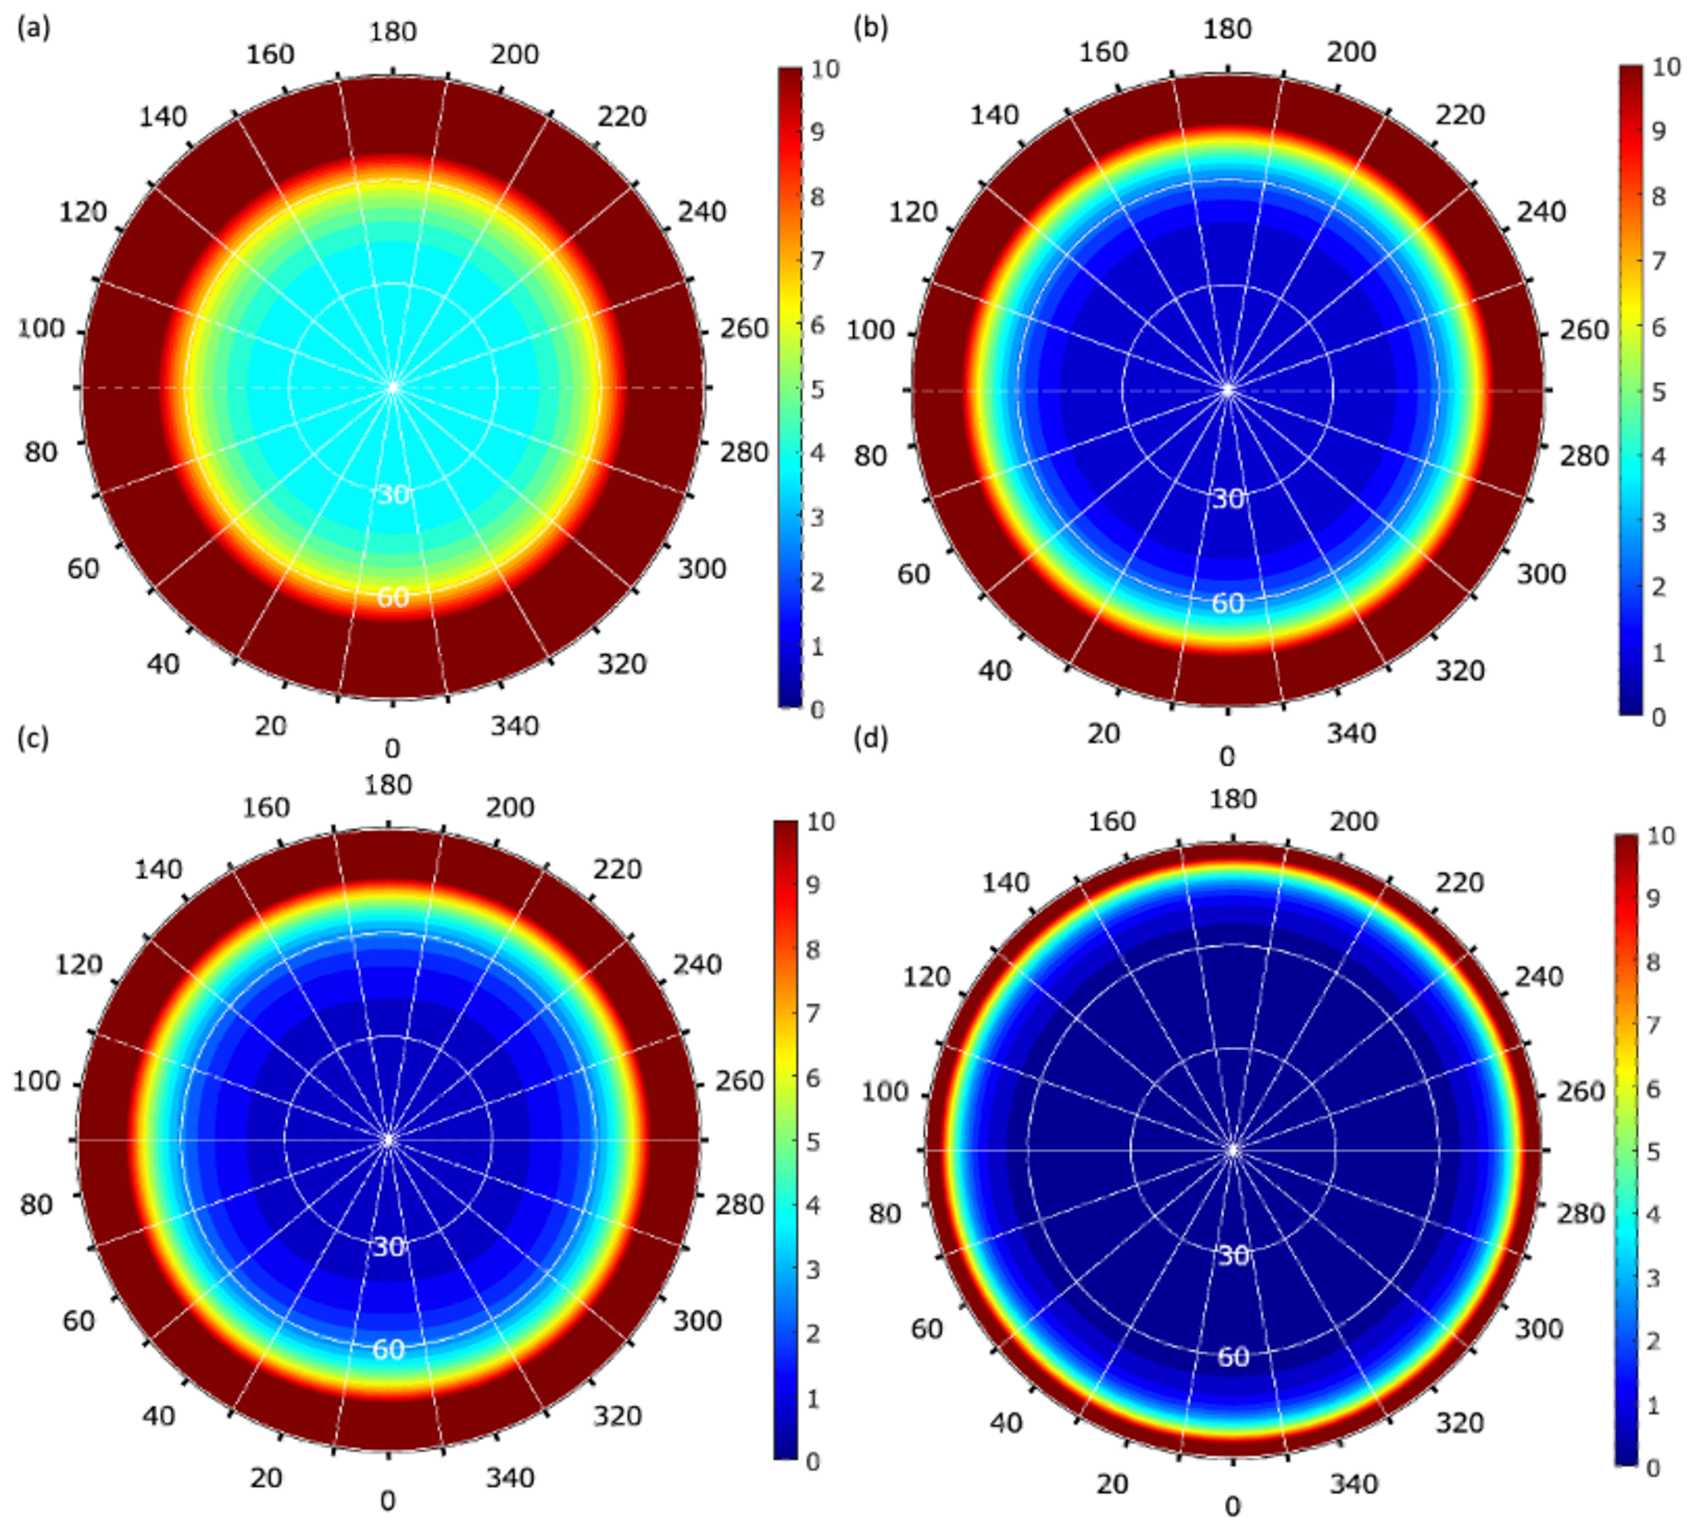
\includegraphics[width=13cm]{AzimuthReflection}
\caption{Polar plots of integrated solar reflection for (a) bare glass, (b) thin film, (c) nanowire array and (b) nanocone array.  
The incidence angle $\theta$ in degrees is shown along the radial direction and the azimuth angle $\gamma_i$ in degrees along the circumference.   }
 \label{fig:AzimuthReflection}
 \end{figure}
 
 Fig.~\ref{fig:AzimuthReflection} plots the solar integrated reflection for the four structures as a function of incidence angle $\theta$ and 
 azimuthal injection angle $\gamma_i$.  
 The bare glass and thin film antireflection layer have no azimuthal angle injection angle dependence, whereas the 
 the NW array and NC arrays both have very weak azimuthal angle injection angle dependence, and thus for simplifying the calculations
 we simply use the averaged azimuthal angle reflection of the different surfaces
\begin{multline}
b_{R} \approx  b_{bn} (\lambda, AM) \tilde{R}(\lambda, \theta) \cos \theta +  b_d (\lambda, AM) \int_{0}^{\pi/2 - \beta} \left ( \frac{1 + \cos \theta}{2} \right ) \tilde{R}(\lambda, \theta) d \theta
\end{multline}
where $\tilde{R}(\lambda, \theta)$ is the averaged reflection over all the azimuth directions.  

 
The total photon flux reflected is
\begin{equation}
\Phi_{R} = \int b_{R} (\lambda) d \lambda
\end{equation}
\begin{align}
%\Phi_{R} (\theta) & \approx \cos \theta + \int b_d (\lambda) \int_{0}^{\pi/2 - \beta} \left ( \frac{1 + \cos \theta}{2} \right ) R(\lambda, \theta) d \theta d \lambda \\
\Phi_{R} (\theta) &= \cos \theta \int b_{bn} (\lambda) R(\lambda, \theta) d \lambda  +  \int_{0}^{\pi/2 - \beta} \left ( \frac{1 + \cos \theta}{2} \right ) \int b_d (\lambda) R(\lambda, \theta) d \lambda d \theta
\end{align}
%where the direct beam photon flux is 
%\begin{equation}
%\Phi_{bn} = \int b_b (\lambda) d \lambda
%\end{equation}



%
%\begin{equation}
%R_s (\theta) = \frac{ \int b_b (\lambda) R(\lambda, \theta) d \lambda }{ \int b_b (\lambda) d \lambda}
%\end{equation}

The annual solar cell flux reflected is 
\begin{equation}
B_{RA} = \frac{12}{\pi} \times 3600 \int_{0}^{365} \int_{-\omega_s} ^{\omega_s} \Phi_{R} (\theta) d \omega d n 
\end{equation}
The annual module reflection is the portion of photons over an entire year that are lost due to 
reflection is 
%reflection
\begin{align}
R_{A} &= \frac{B_{RA}}{B_{mA}} \\
\end{align}


% The annual average daily total module insolation is
% \begin{align}
% H_{Tm} = \frac{1}{365} \int_0^{365} \frac{12}{\pi} \int_{-\omega_s}^{\omega_s}  I_{Tm} d \omega d n    
% \end{align}
% %where $\omega$ is the hour angle.
% where $\omega_s$ is the sunset hour angle
% \begin{align}
%  \omega_s &= \cos^{-1} \left ( - \tan \phi \tan \delta \right ) 
% \end{align}
% and $-\omega_s$ is the sunrise hour angle.
% $\omega = 0$ at solar noon.  

%The number of incident photons through the glass/air interface
%%not reflected by the glass/air interface is
%%module is
%\begin{multline}
%b_{Tc} =  b_{bn} (\lambda)  \left [ 1 - R(\lambda, \theta, \gamma_i) \right ]  + \\ 
%b_d \frac{1}{2 \pi } \int_{0}^{2 \pi} \int_{0}^{\pi/2 - \beta} \left ( \frac{1 + \cos \theta}{2} \right ) \left [ 1 - R(\lambda, \theta, \gamma_i)  \right ] d \theta d \gamma
%\end{multline}
%where $R(\lambda, \theta, \gamma_i)$ is the reflection spectra of the module/interface is a function of 
%angle of incidence $\theta$, and injection azimuth angle $\gamma_i$. 
%$\gamma_i = \gamma - \gamma_s$, where $\gamma$ is the module azimuth angle and $\gamma_s$ is the solar azimuth angle.  
%The azimuth angle is defined so $0 \degree$ is south,   negative is east, and positive is west \cite{Duffie:13}.  
%The total photon flux transmitted through the top glass is 
%\begin{equation}
%\Phi_{Tc} = \int b_{Tc} (\lambda) d \lambda
%\end{equation}
%The annual solar cell flux is 
%\begin{equation}
%B_{cA} = \frac{12}{\pi} \times 3600 \int_{0}^{365} \int_{-\omega_s} ^{\omega_s} \Phi_{Tc} d \omega d n 
%\end{equation}
%The annual module reflection is the portion of photons over an entire year that are lost due to 
%reflection is 
%%reflection
%\begin{align}
%R_{A} &= \frac{B_{mA} - B_{cA} }{B_{mA}} \\
%&= \frac{B_{mA} - \left [ B_{mA} - B_{RA} \right ] }{B_{mA}} \\
%&= \frac{B_{RA} }{B_{mA}} \\
%\end{align}








% where the air mass $AM$ is defined as 
% \begin{equation}
% AM (\omega, \delta, \gamma_s) = \frac{1}{cos\left [ \theta_z (\omega, \delta, \gamma_s) \right ]}.
% \end{equation}

% $\theta_z$ is the zenith angle of the sun, 
% $\omega$ is the hour angle, and $\delta$ is declination angle, and $\gamma$ is the module angle.
%whereωis the hour angle and $\delta$ is the %latitude.
%where 






%% The Appendices part is started with the command \appendix;
%% appendix sections are then done as normal sections
%% \appendix

%% \section{}
%% \label{}

%% If you have bibdatabase file and want bibtex to generate the
%% bibitems, please use
%%
%%  \bibliographystyle{elsarticle-num} 
%%  \bibliography{<your bibdatabase>}

%% else use the following coding to input the bibitems directly in the
%% TeX file.

%\begin{thebibliography}{00}
%
%%% \bibitem{label}
%%% Text of bibliographic item
%
%\bibitem{}

\section{Data Availability}

All python code used for the model to generate the figures in the manus-cript can be found in the following Github repository: \\ \url{https://github.com/pleu/LAMPsolar}.

\section{Acknowledgements}
This work was supported by the National Science Foundation [grant number 1930582].

\bibliographystyle{elsarticle-num}
\bibliography{LAMPPapers,AllRefs}


%\end{thebibliography}
\end{document}
\endinput
%%
%% End of file `elsarticle-template-num.tex'.
